\documentclass[a4paper,12pt]{report}
\usepackage[fiche,niveau={1MA1},nfiche={17}, annee={Emilie-Gourd, 2024--2025}, auteur={ns},theme={Fonctions -- Paraboles}]{packages/bandeaux}
\usepackage{packages/boites}
\usepackage{packages/fontes}
\usepackage{packages/courslatex}
\usepackage{packages/mathenv}
\allowdisplaybreaks

\begin{document}
\pgfplotsset{every axis/.append style={
                    axis x line=middle,
                    axis y line=middle,
                    axis line style={->},
                    xlabel={$x$},
                    ylabel={$y$},
                    label style={font=\small},
                    tick label style={font=\small},
                    unit vector ratio*=1 1 1,
   					xlabel style={at={(ticklabel* cs:1)},anchor=north west},
   					ylabel style={at={(ticklabel* cs:1)},anchor=south west}
                    }}
{\bfseries Compétences :}
\begin{itemize}
	\item Déterminer le sommet d'une parabole
	\item Déterminer les zéros d'une parabole
	\item Déterminer l'axe de symétrie d'une parabole
	\item Utiliser les différentes écritures d'une parabole : forme générale, forme canonique, forme factorisée
\end{itemize}

\begin{defi}[parabole]
La courbe représentative d'une fonction de degré 2 s'appelle une {\bfseries parabole}. Une la représentation d'une fonction de degré 2 de la forme $f(x)=ax^2+bx+c$ où $a\neq 0$ et $a,b,c\in \mathbb{R}$ est une parabole $y=ax^2+bx+c$. Une parabole peut s'écrire sous différentes formes : forme générale, forme canonique, forme factorisée.
\end{defi}

Avant d'introduire ces trois écritures, nous devons définir les notions suivantes. 

\begin{defi}[zéros]
	Les {\bfseries zéros} d'une parabole sont les points d'intersection de la parabole avec l'axe des abscisses. Ce sont les solutions de l'équation $ax^2+bx+c=0$.
\end{defi}

\begin{defi}[sommet]
	Le {\bfseries sommet} d'une parabole, noté $S$, est le point de la parabole qui a l'ordonnée minimale (si $a>0$) et maximale (si $a<0$).
\end{defi}
   
\begin{rem}
Pour une parabole $f(x)=ax^2+bx+c, a\neq 0$, le sommet est donné par les coordonnées 
\[\left(-\dfrac{b}{2a};f\left(-\dfrac{b}{2a}\right)\right).\]
\end{rem}

    \begin{defi}[Axe de symétrie d'une parabole]
	    L'{\bfseries axe de symétrie} d'une parabole est la droite qui partage la parabole en deux parties symétriques. 
    \end{defi}
    \begin{rem}
    Pour une parabole $y=ax^2+bx+x, a\neq 0$, l'axe de symétrie est donné par l'équation $x=-\dfrac{b}{2a}$.
    \end{rem}
    
    \begin{defi}[forme générale d'une parabole]
	    La {\bfseries forme générale} d'une parabole est donnée par $y=ax^2+bx+c$.
    \end{defi}
    
    \begin{defi}[forme canonique d'une parabole]
	    La {\bfseries forme canonique} d'une parabole est donnée par $y=a(x-\alpha)^2+\beta$ où $(\alpha;\beta)$ est le sommet de la parabole.
    \end{defi}

    \begin{defi}[forme factorisée d'une parabole]
	    La {\bfseries forme factorisée} d'une parabole est donnée par $y=a(x-x_1)(x-x_2)$ où $x_1$ et $x_2$ sont les zéros de la parabole.
    \end{defi}
    
    \begin{rem}
    	Pour passer de la forme générale à la forme canonique, on peut utiliser deux méthodes : 
	\begin{enumerate}
		\item Calcul du sommet par la formule \[S\left(-\dfrac{b}{2a};f\left(-\dfrac{b}{2a}\right)\right)\] et substition dans la forme canonique : 
        \[y=\left(x+\dfrac{b}{2a}\right)+f\left(-\dfrac{b}{2a}\right)\]
\item Complétion du carré :

       \begin{align*}
        &y=ax^2+bx+c\\
        &y=a\left(x^2+\dfrac{b}{a}x\right)+c\\
        &y=a\left(x^2+ \dfrac{b}{a}x+\dfrac{b^2 }{4a^2 }-\dfrac{b^2 }{4a^2 }\right)+c\\
        &y=a\left(x+\dfrac{b}{2a}\right)^2 -\dfrac{b^2 }{4a}+c\\
	&y=a\left(x+\dfrac{b}{2a}\right)^2 -\dfrac{b^2 -4ac}{4a}\\
        \end{align*}
	\end{enumerate}
    \end{rem}
    \begin{rem}
    Pour passer de la forme générale à la forme factorisée, on utilise les zéros de la parabole. Les zéros sont les solutions de l'équation $ax^2+bx+c=0$. 

Si $\Delta\geq 0$. On a $x_1=\dfrac{-b-\sqrt{b^2-4ac}}{2a}$ et $x_2=\dfrac{-b+\sqrt{b^2-4ac}}{2a}$. Ainsi, la forme factorisée est donnée par \[y=a(x-x_1)(x-x_2).\]
    \end{rem}
    \begin{boiteExT}[Étude de la parabole $f(x)=\dfrac{3}{2}x^2-\dfrac{3}{2}x-3$]
	\vspace{10cm}
\end{boiteExT}
\begin{exo}
	Déterminer la forme canonique de chacun des polynômes définis par :
	\begin{tasks}(3)		
\task $R(x)=-2 x^2+8 x-11$
\task $S(x)=-3 x^2-30 x-70$
\task $T(x)=-4 x^2-32 x-68$
	\end{tasks}
\end{exo}
\begin{exo}
	Pour les paraboles suivantes, déterminer les zéros de la parabole, l'axe de symétrie, la forme canonique et la forme factorisée
	\begin{tasks}(3)
\task $f(x)=3 x^2-2 x-1$
\task $g(x)=-\frac{2}{3} x^2+4 x-3$
\task $h(x)=x^2-4 x+5$
\end{tasks}
\end{exo}
\newpage
    {\bfseries Compétences :}
 \begin{itemize}
	 \item Établir un tableau de signes d'une parabole
	 \item Réaliser une étude complète d'une parabole
 \end{itemize}

 Dans cette fiche, nous verrons comment utiliser ce que nous avons vu précédemment pour réaliser une étude complète d'une parabole. Nous commençons par organiser les données dans un tableau de signes.

 \begin{defi}[tableau de signes]
	 Un {\bfseries tableau de signes} est un tableau qui permet de lire rapidement la variation des signes d'une fonction.
 \end{defi}
        
 \begin{rem}
	 Pour réaliser un tableau de signes, on commence par déterminer les zéros de la parabole. On place sur la première ligne les zéros dans un tableau avec des bornes $-\infty$ et $+\infty$ aux extrémités. On évalue la parabole pour des valeurs dans les intervalles délimités par les zéros pour obtenir le signe de la parabole dans cet intervalle. On peut aussi utiliser nos connaissances sur les variations de la fonction pour déterminer les signes.
 \end{rem}
 
 
\begin{boiteExT}[Tableau de signes de la parabole $f(x)=x^2-3x+2$]
	\vspace{8cm}
\end{boiteExT}

\begin{exo}
	Dresser le tableau de signes des signes des fonctions suivantes :
	\begin{tasks}(3)
	\task $f(x)=(x-5)(x+4)$.
 \task $g(x)=2(x-5)(x-7)$.
 \task $h(x)=-6(x+5)(x+1)$.
	\end{tasks}
\end{exo}
	\begin{exo}
		Réaliser une étude complète et représenter graphiquement la parabole $f(x)=-2 x^2-\dfrac{21}{5} x-\dfrac{9}{5}$
	\end{exo}
\newpage
   \begin{rem}
   Pour réaliser une étude complète d'une parabole, il faut:
   \begin{enumerate}
	   \item Déterminer les zéros de la parabole
\item Déterminer le point d'intersection avec l'axe des ordonnées
\item Détermine ensuite l'axe de symétrie
\item Déterminer le sommet de la parabole
\item Déterminer la concavité et réaliser un tableau de signes
\item Utiliser les informations pour représenter graphiquement la parabole (plaçant les points particuliers et en utilisant le tableau de signes).
\end{enumerate}
   \end{rem}
 
   \begin{boiteExT}[Étude complète de la paraoble $f(x)=-x^2+3x-2$]
	   \vspace{18cm}
\end{boiteExT}
\begin{boiteicone}
	Soyez le plus précis possible dans la représentation graphique~!
\end{boiteicone}
\newpage
\begin{center}
	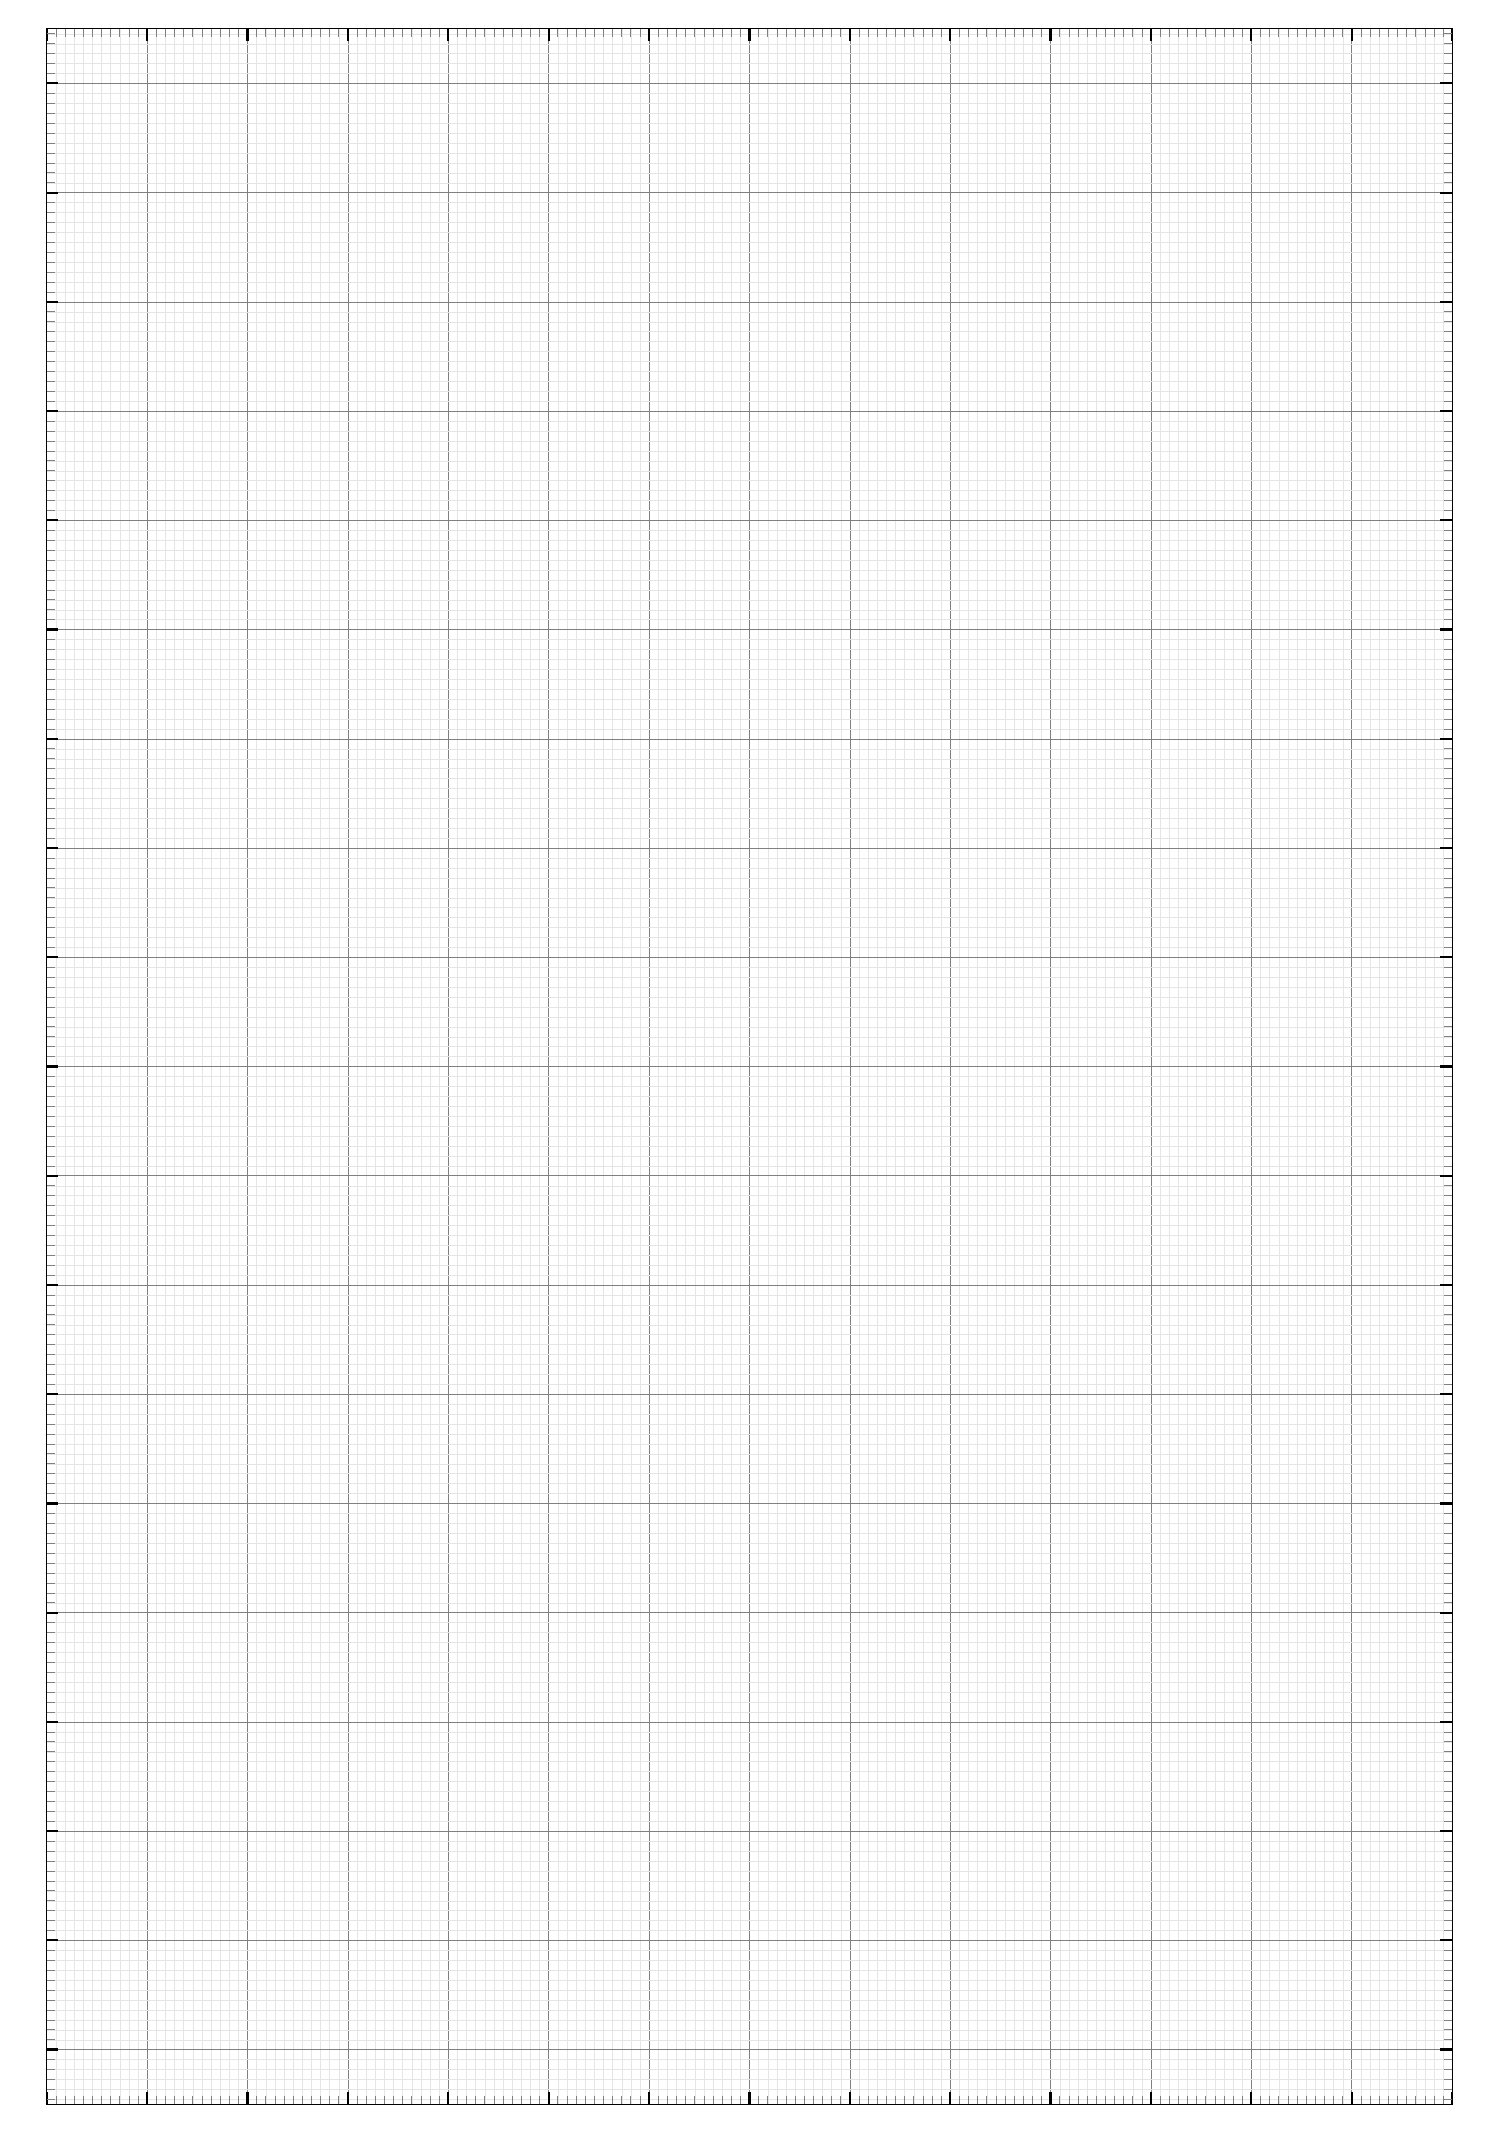
\begin{tikzpicture}

   \begin{axis}[
  width=\paperwidth*0.9,
  height=\paperheight,
	 name = graph1,
     ytick distance = 1,
     xtick distance = 1,
     ymin=-9.5, ymax=9.5,
     xmin=-7, xmax=7,
     grid=both,
     grid style={line width=.1pt,draw=black!10},
     major grid style={line width=.2pt,draw=black!50},
     minor tick num=10,
	major tick style={
    thick,          % Predefined thick style
    color=black,    % Tick color
},
         xticklabel=\empty, % Removes x-axis numerical labels
        yticklabel=\empty, % Removes y-axis numerical labels    tick label={draw=none},
   ]
   \end{axis}
  \end{tikzpicture}
\end{center}
\newpage
\begin{center}
	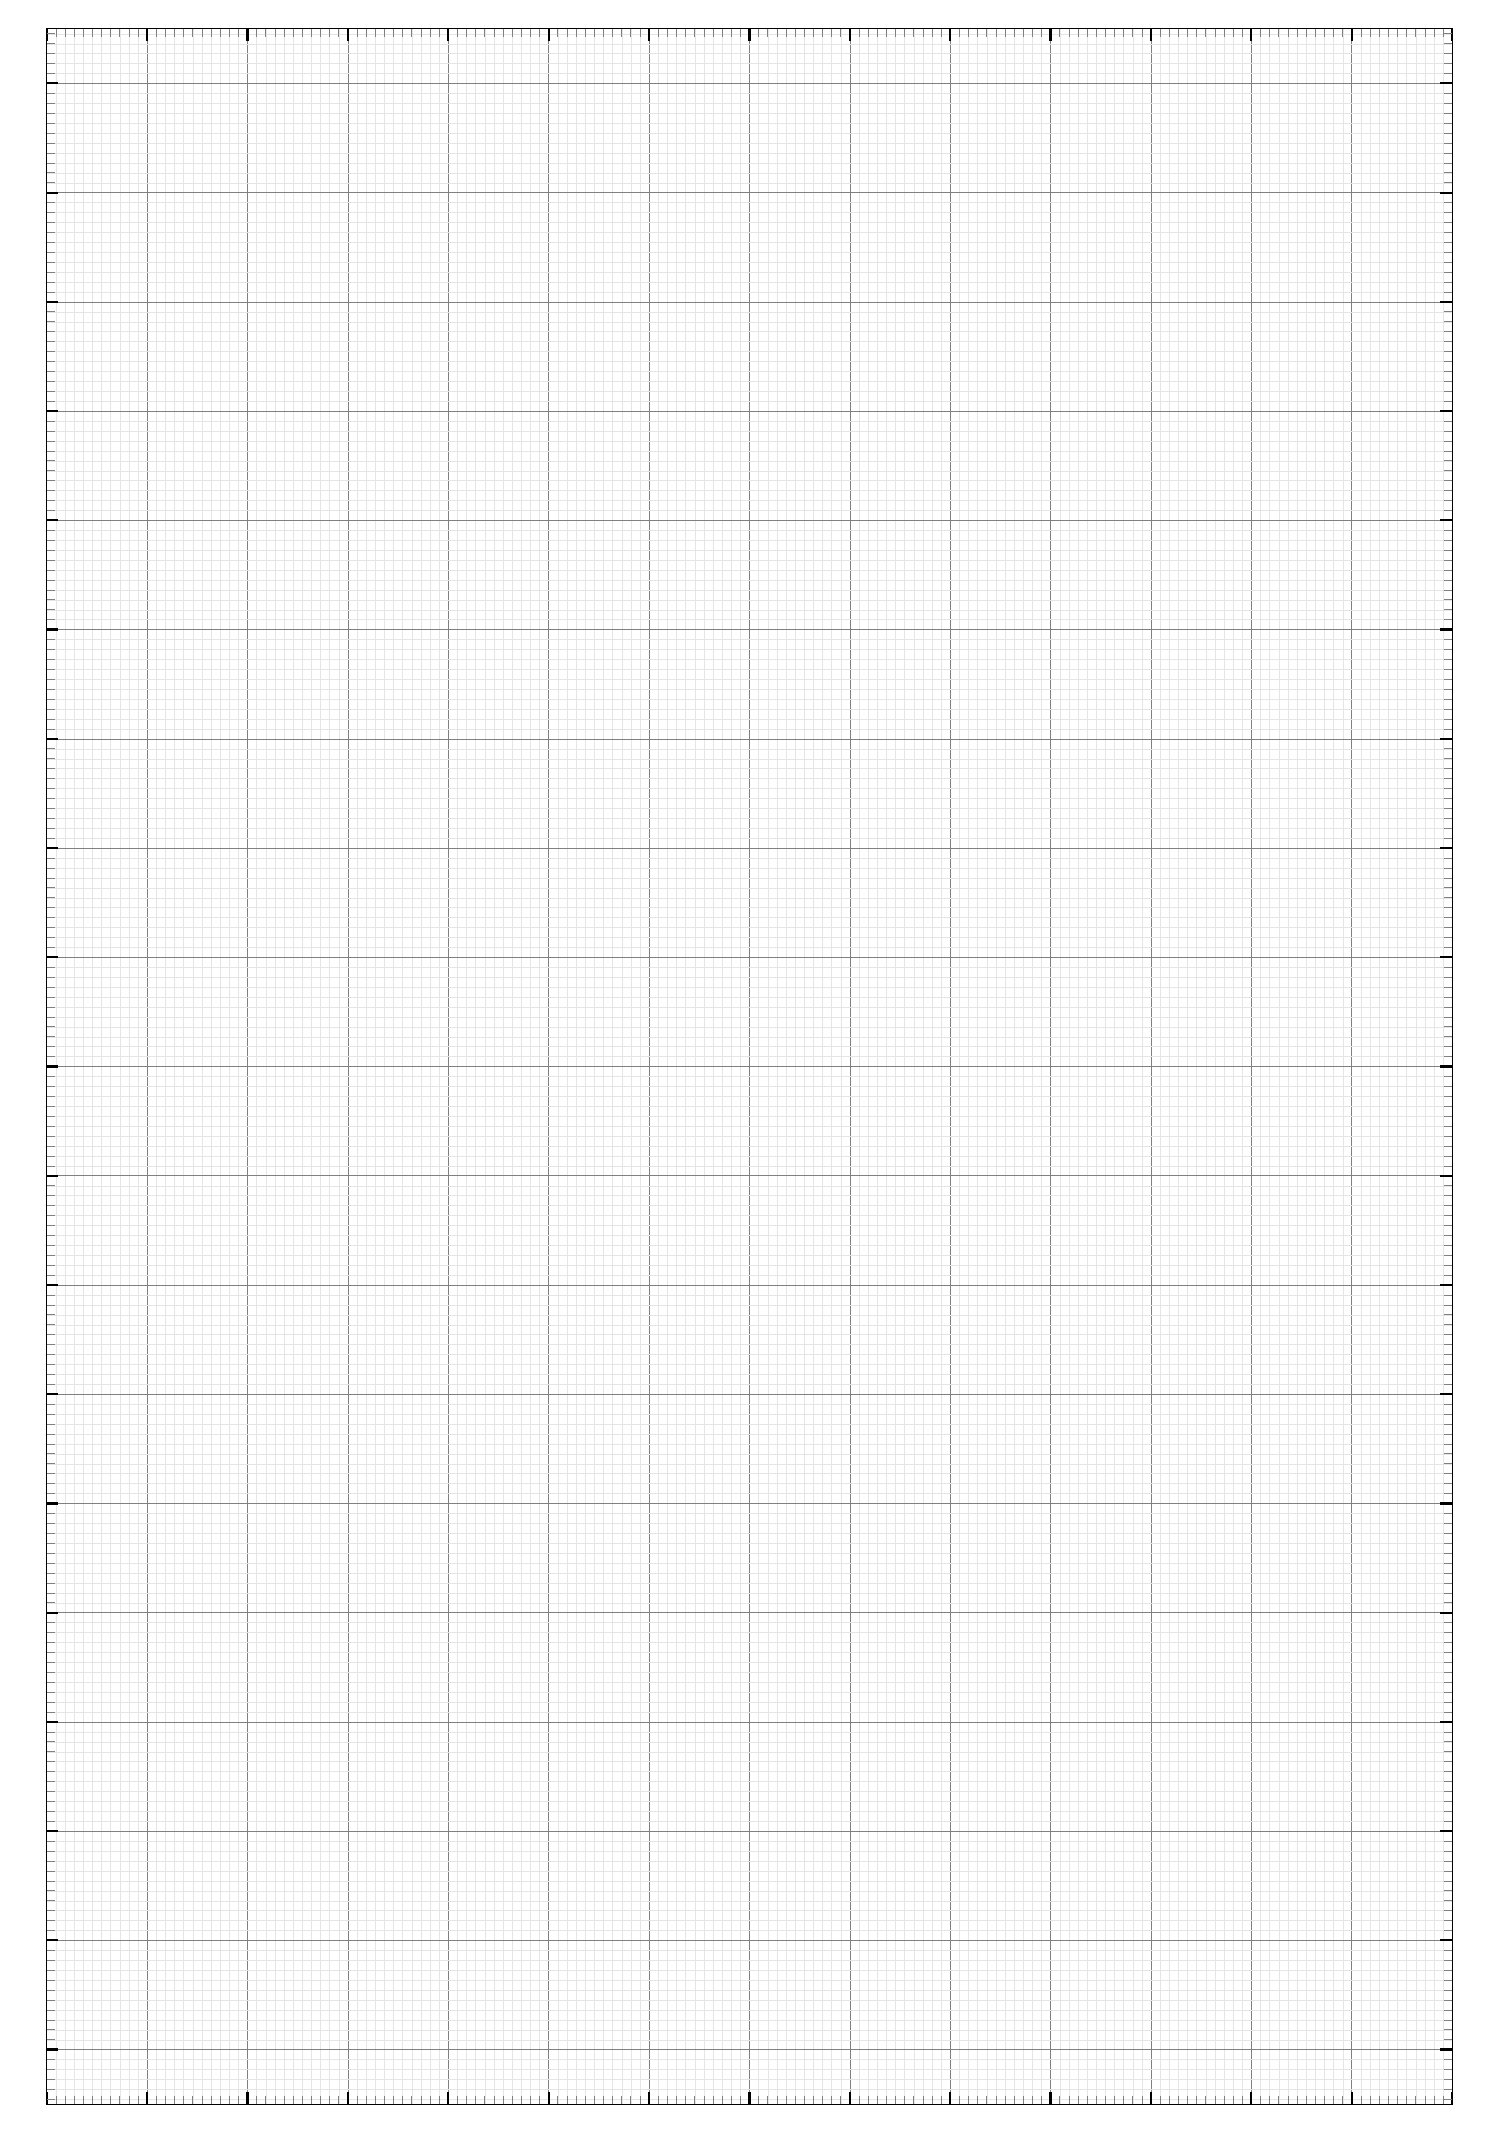
\begin{tikzpicture}

   \begin{axis}[
  width=\paperwidth*0.9,
  height=\paperheight,
	 name = graph1,
     ytick distance = 1,
     xtick distance = 1,
     ymin=-9.5, ymax=9.5,
     xmin=-7, xmax=7,
     grid=both,
     grid style={line width=.1pt,draw=black!10},
     major grid style={line width=.2pt,draw=black!50},
	major tick style={
    thick,          % Predefined thick style
    color=black,    % Tick color
},
         xticklabel=\empty, % Removes x-axis numerical labels
        yticklabel=\empty, % Removes y-axis numerical labels    tick label={draw=none},
     minor tick num=10,
   ]
   \end{axis}
  \end{tikzpicture}
\end{center}
\newpage
\begin{center}
	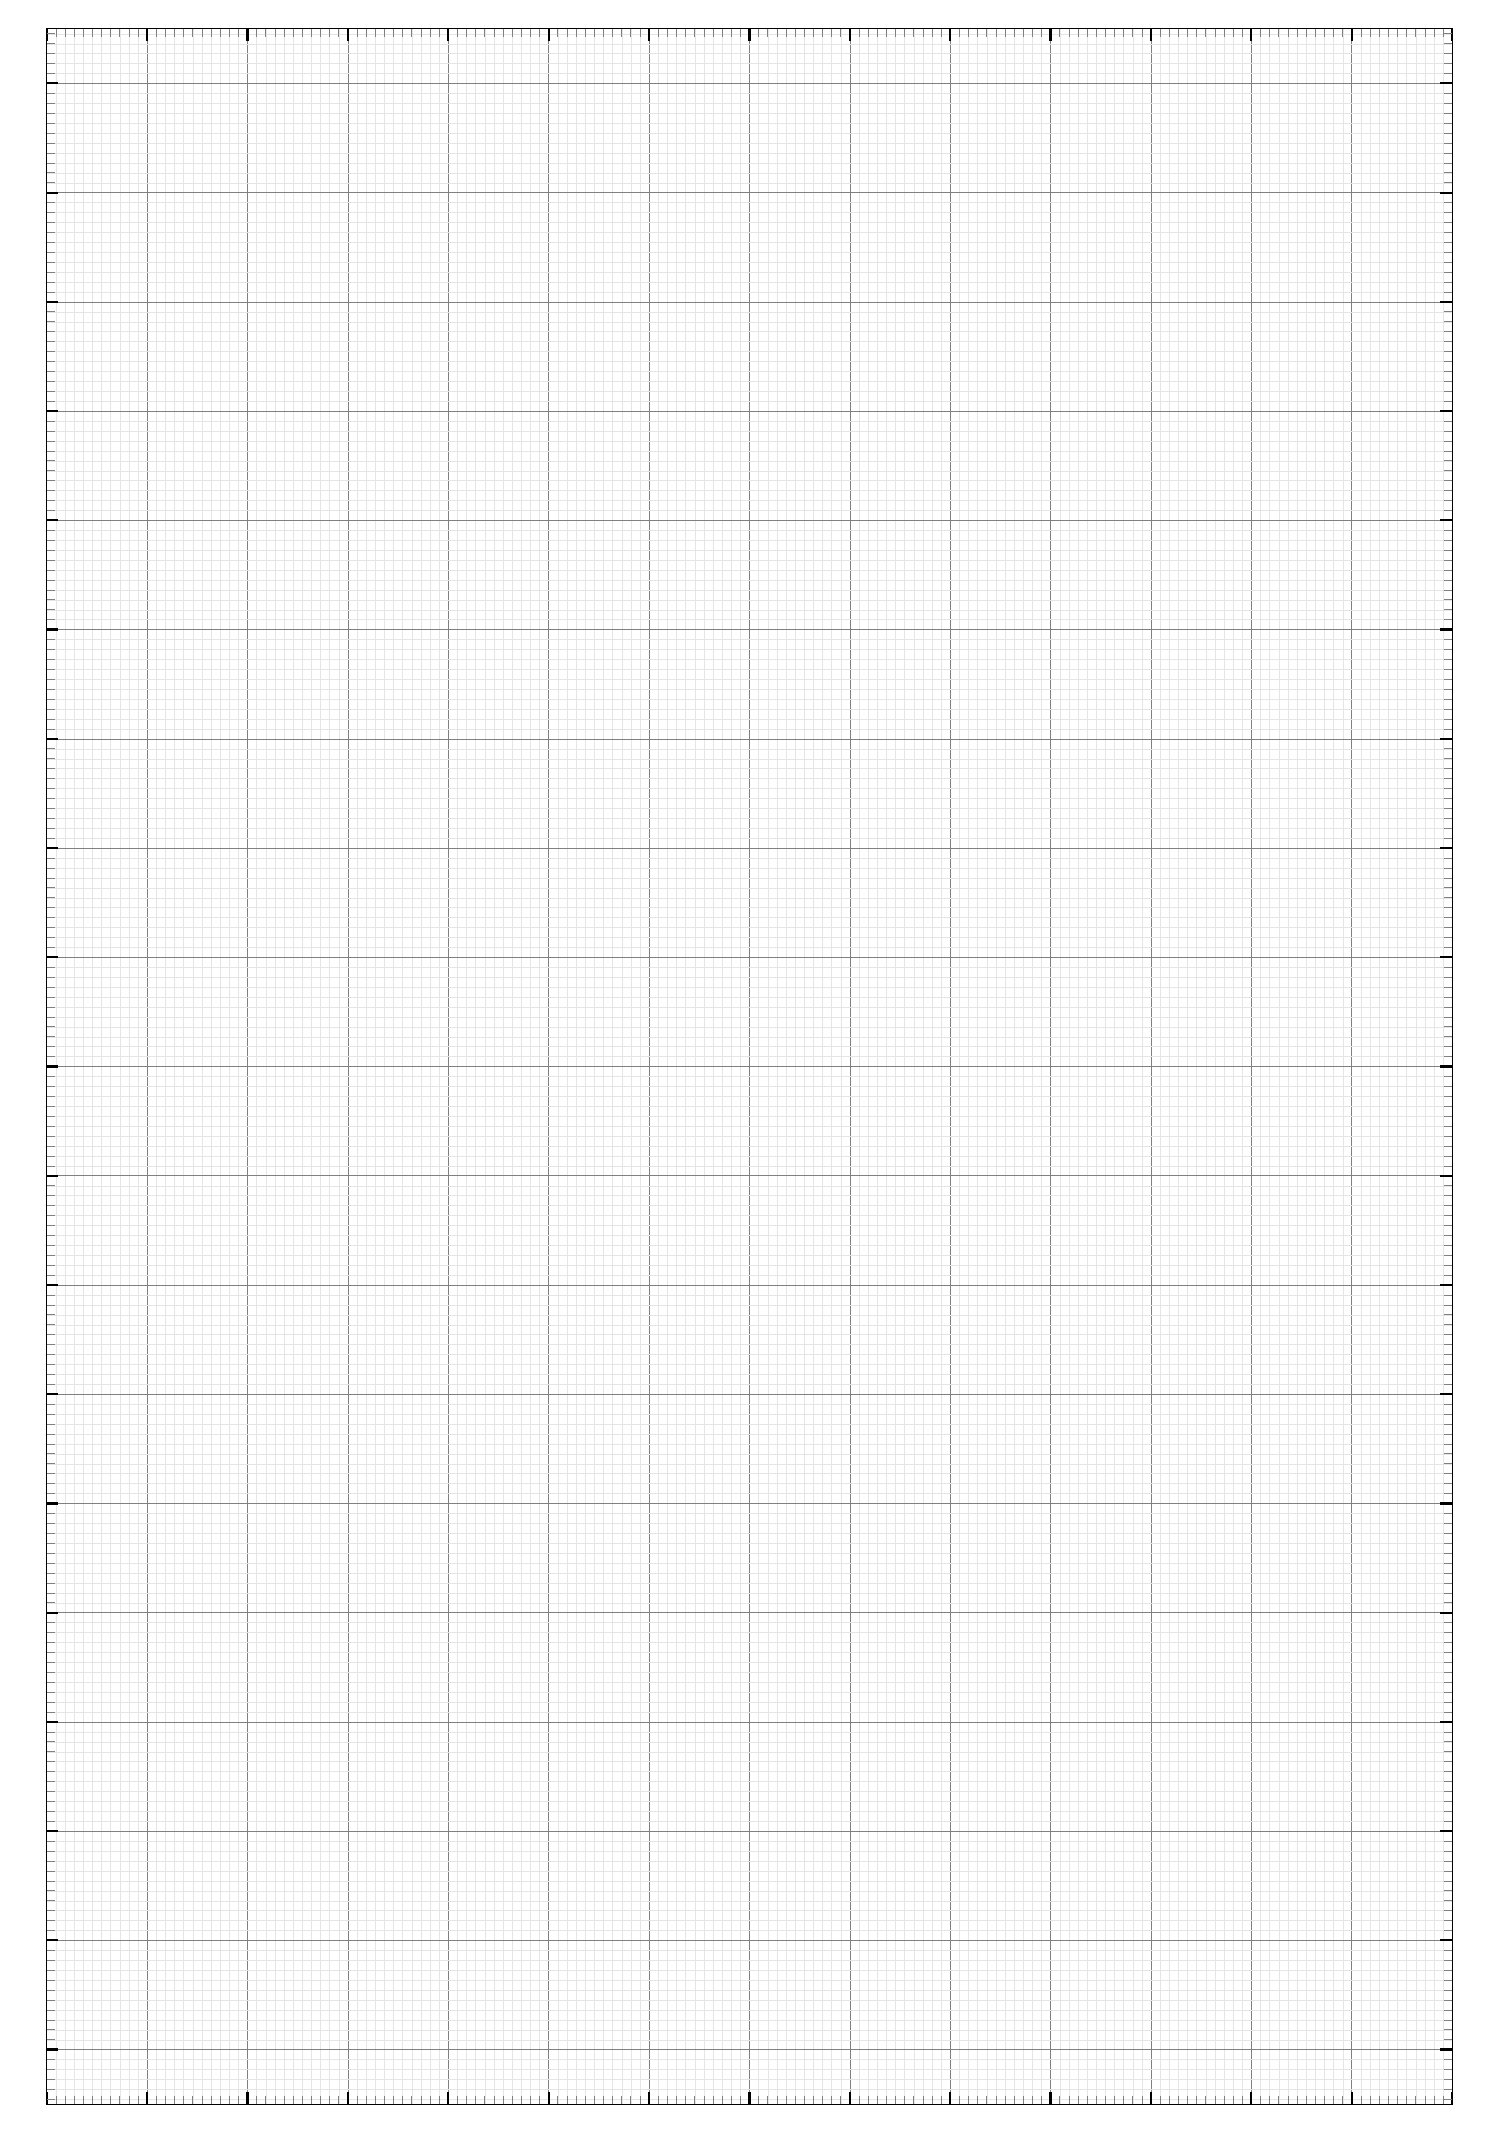
\begin{tikzpicture}

   \begin{axis}[
  width=\paperwidth*0.9,
  height=\paperheight,
	 name = graph1,
     ytick distance = 1,
     xtick distance = 1,
     ymin=-9.5, ymax=9.5,
     xmin=-7, xmax=7,
     grid=both,
     grid style={line width=.1pt,draw=black!10},
     major grid style={line width=.2pt,draw=black!50},
     minor tick num=10,
	major tick style={
    thick,          % Predefined thick style
    color=black,    % Tick color
},
         xticklabel=\empty, % Removes x-axis numerical labels
        yticklabel=\empty, % Removes y-axis numerical labels    tick label={draw=none},
   ]
   \end{axis}
  \end{tikzpicture}
\end{center}
\newpage
\begin{center}
	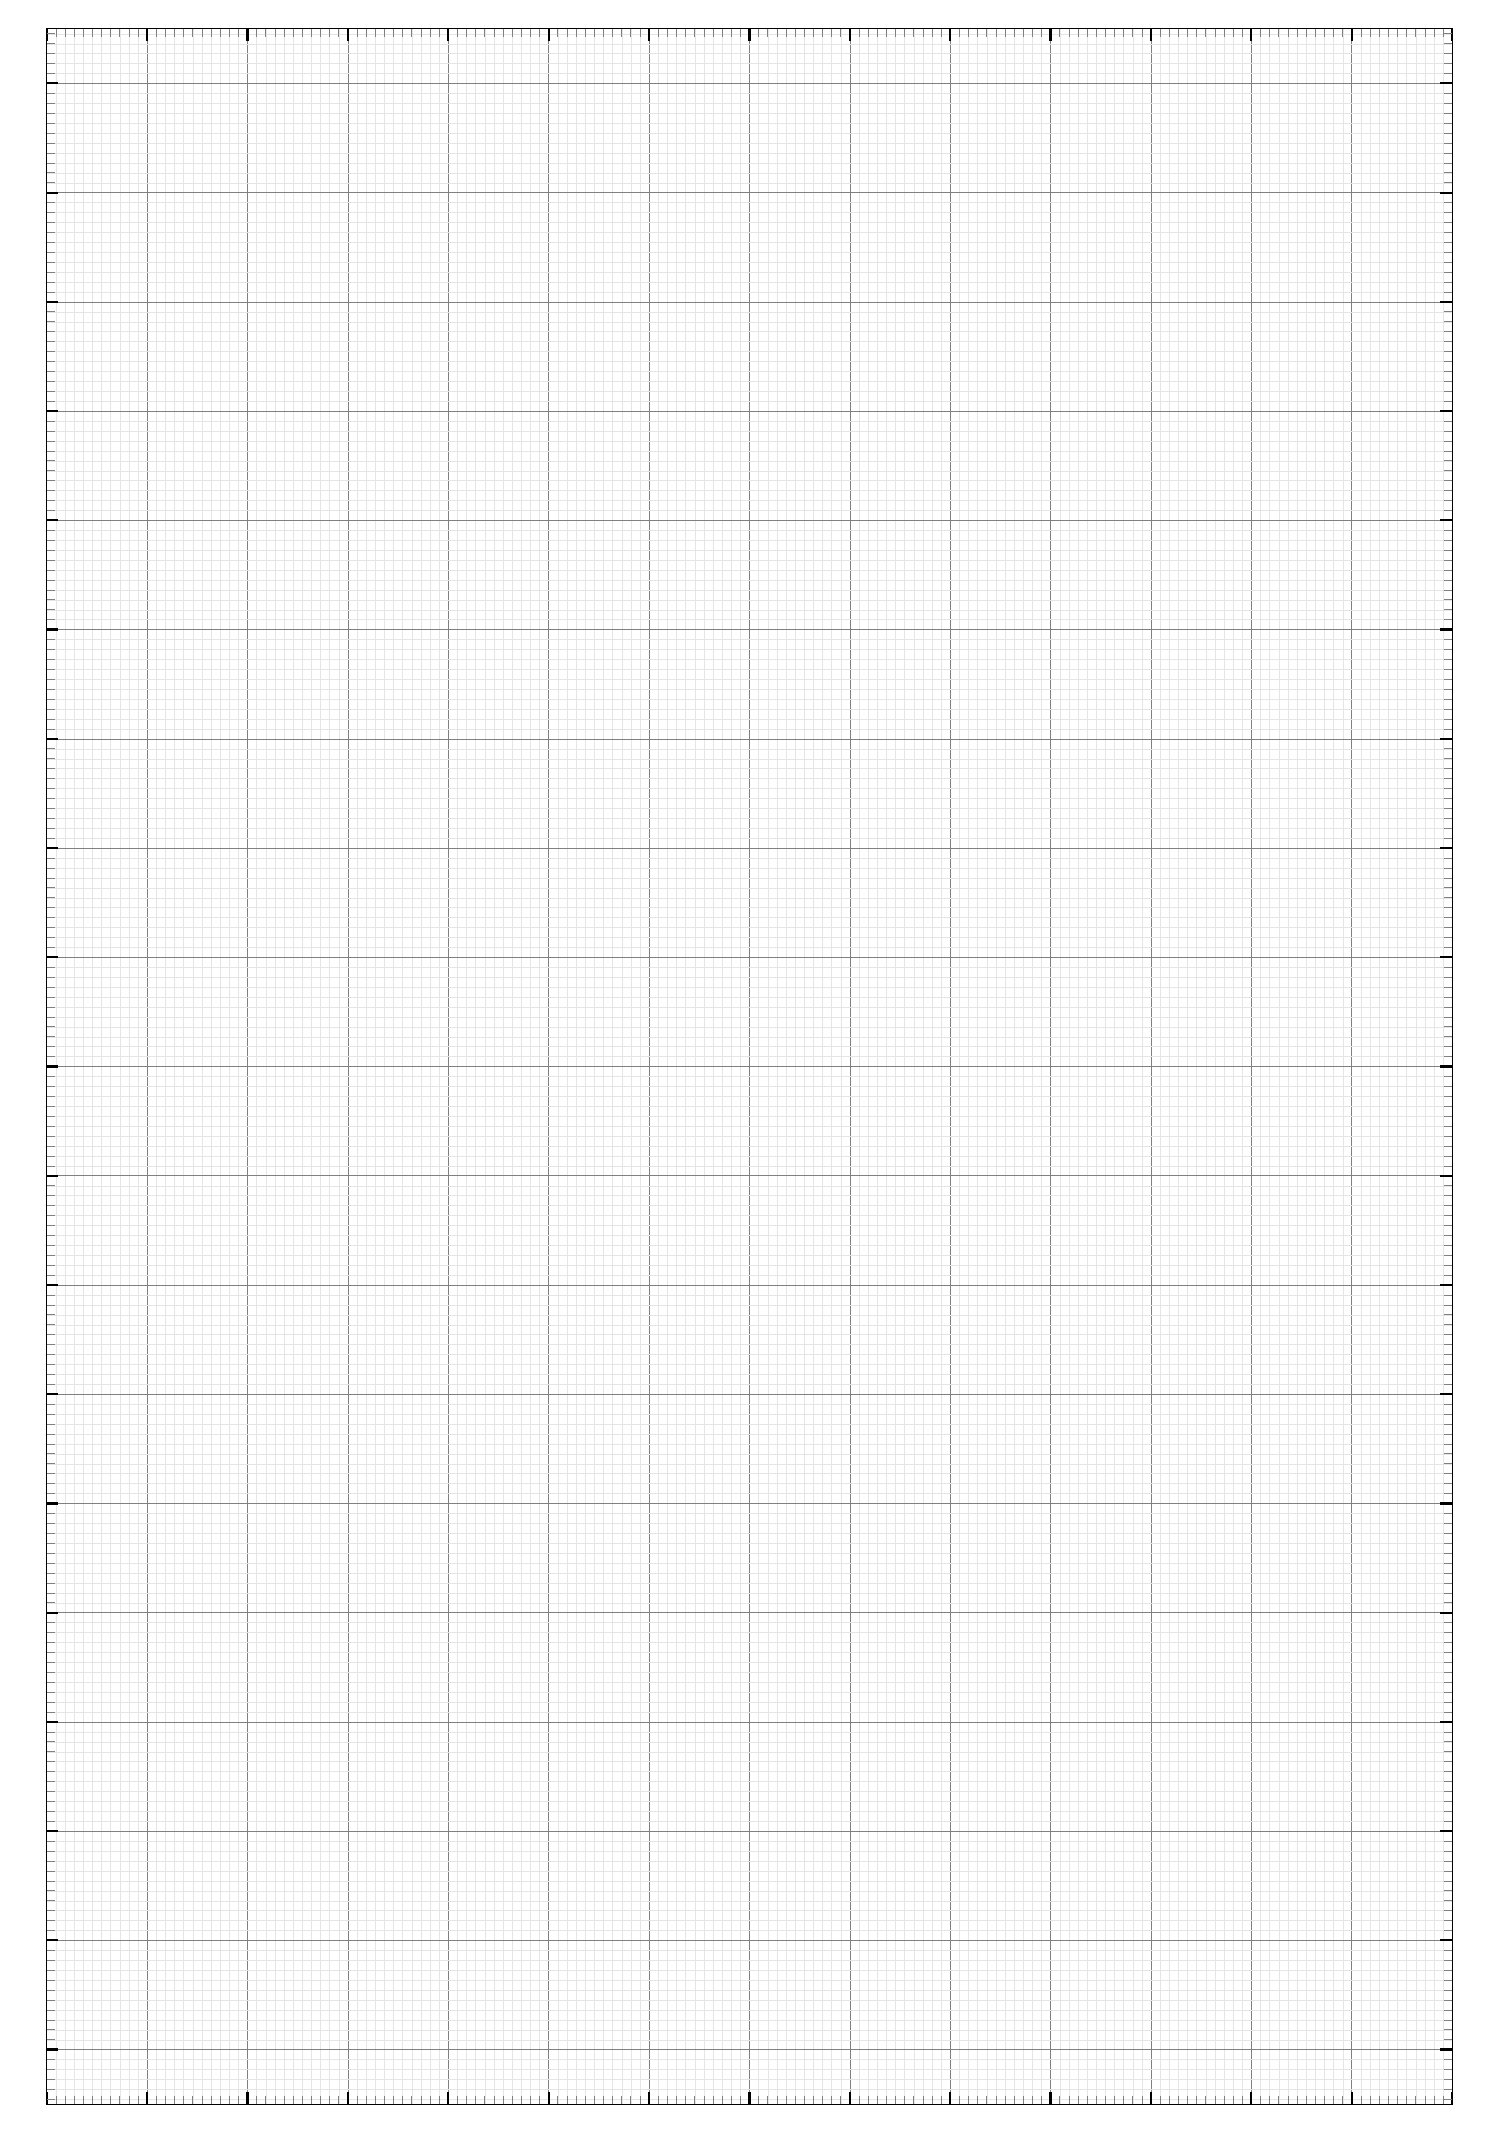
\begin{tikzpicture}

   \begin{axis}[
  width=\paperwidth*0.9,
  height=\paperheight,
	 name = graph1,
     ytick distance = 1,
     xtick distance = 1,
     ymin=-9.5, ymax=9.5,
     xmin=-7, xmax=7,
     grid=both,
     grid style={line width=.1pt,draw=black!10},
     major grid style={line width=.2pt,draw=black!50},
     minor tick num=10,
	major tick style={
    thick,          % Predefined thick style
    color=black,    % Tick color
},
         xticklabel=\empty, % Removes x-axis numerical labels
        yticklabel=\empty, % Removes y-axis numerical labels    tick label={draw=none},
   ]
   \end{axis}
  \end{tikzpicture}
\end{center}
\end{document}


